% IKT 2026 English paper.
% Source: IEEE conference template dated 6/27/2024 (IEEEtran.cls in this folder).
% Paper size is A4, matching IKT_Template_(English).doc.
% If IEEE PDF eXpress later asks for US Letter, delete the a4paper option.
%
% Recent IKT English limits were 5 pages, or up to 7 pages with an extra-page
% fee, including figures, tables, and references. Confirm the 2026 limit.
% Do not change margins, column widths, fonts, or line spacing.
% Do not use symbols, special characters, footnotes, or math in the title
% or the abstract. Subtitles are dropped by IEEE Xplore; do not add one.
%
% Build from this folder:
%   pdflatex main
%   bibtex main
%   pdflatex main
%   pdflatex main

\documentclass[conference,a4paper]{IEEEtran}

% Uncomment the next line only if you add a \thanks funding footnote.
% \IEEEoverridecommandlockouts

\usepackage{cite}
\usepackage{amsmath,amssymb,amsfonts}
\usepackage{algorithmic}
\usepackage{graphicx}
\usepackage{textcomp}
\usepackage{xcolor}

% The stock IEEEtran conference class leaves the running header empty.
% IKT's Word template adds this line to the first page only, centered,
% in 10 pt Times, and puts the IEEE copyright placeholder in the first-page
% footer. Later pages have neither. Camera-ready submission replaces the
% footer with the copyright line IEEE assigns.
\makeatletter
\def\ps@IEEEtitlepagestyle{%
  \def\@oddhead{\hfil\normalfont\normalsize
    2026 17th International Conference on Information and Knowledge Technology (IKT)\hfil}%
  \let\@evenhead\@empty
  \def\@oddfoot{\normalfont\normalsize
    xxxx-..-\textellipsis.-\textellipsis.-x/xx/\$xx.00~\copyright2026IEEE\hfil}%
  \let\@evenfoot\@empty}
\makeatother

\begin{document}

\title{Comparing Forecasters for Serverless Invocation Provisioning}

% Funding footnote, if any. Delete it when there is no sponsor.
% \thanks{Identify the funding agency here.}

\author{\IEEEauthorblockN{Ehsan Moradi}
\IEEEauthorblockA{\textit{Department of Computer Engineering} \\
\textit{Amirkabir University of Technology}\\
Tehran, Iran \\
your.email@aut.ac.ir}
% \and
% \IEEEauthorblockN{Seyyed Ahmad Javadi}
% \IEEEauthorblockA{\textit{Department of Computer Engineering} \\
% \textit{Amirkabir University of Technology}\\
% Tehran, Iran \\
% email address or ORCID}
}

\maketitle

\begin{abstract}
Serverless platforms keep warm containers ready for a changing arrival rate. Too few containers cause cold starts, and too many sit idle. This paper compares six forecasters of per-minute function invocations on a public Azure Functions trace: three simple baselines, seasonal Holt--Winters, a pretrained time-series model, and a small LSTM. Functions are grouped into sparse, daily, bursty, and other workloads. Each forecast covers the next 60 minutes, and the fitted models see the previous day. Error is reported with a provisioning cost that counts missed invocations and extra container-minutes. On a typical function, copying the previous day has the lowest error. A high percentile of recent load misses fewer invocations and holds more idle capacity. Seasonal smoothing, Chronos-Bolt, and the LSTM remain well above that copy on daily functions. A rule that picks the lowest-shortfall model in each class selects seasonal smoothing for sparse functions on a margin of a fraction of an invocation, and on later days that choice wastes about 1,600 container-minutes with no shortfall gain.
\end{abstract}

\begin{IEEEkeywords}
serverless computing, workload forecasting, cold start, provisioning
\end{IEEEkeywords}

\section{Introduction}
\label{sec:introduction}
A serverless platform receives a changing number of function invocations and must decide how many warm containers to keep. A shortfall makes some requests wait for a cold start. Spare containers consume memory and money while they sit idle. A forecast of the next hour can drive that decision, but a lower forecast error does not by itself mean a better operating point. Under-predicting and over-predicting have different costs.

Forecasting is already part of production resource management. The public Azure Functions study uses a time-series forecast inside a larger keep-alive policy \cite{shahrad2020serverless}. What is still easy to miss is that functions are not one workload. A timer with a daily shape, a rarely called HTTP function, and a bursty queue consumer can prefer different forecasters. Average error over the whole trace hides that split.

This paper is a comparative study, not a new scheduler. On 80 functions from the 2019 Azure Functions invocation trace, it asks which forecaster an operator should use for which class of function, and what that choice costs in missed invocations versus idle containers. The fitted models all see the previous day, so a daily pattern is inside their window. The contributions are a class-aware comparison, a provisioning score beside forecast error, and a selection rule fit on two days and checked on the next two.

\section{Related Work}
\label{sec:related}
Shahrad et al.\ characterize the Azure Functions workload and show that most functions are invoked rarely \cite{shahrad2020serverless}. Their hybrid policy keeps containers warm from a histogram of idle times and falls back to a time-series forecast when the histogram does not cover the idle gaps. This paper uses the same public invocation counts. It does not reimplement that keep-alive policy. The decision here is the number of containers implied by a forecast of arrivals, under a fixed service rate.

Chronos trains a probabilistic forecaster on a large collection of time series and can forecast a new series without retraining \cite{ansari2024chronos}. Chronos-Bolt is a faster variant that emits quantile forecasts for the whole horizon in one pass. We use the small Chronos-Bolt checkpoint with no fine-tuning, and we score its median and two upper quantiles. Upper quantiles are a direct way to buy fewer shortfalls by preparing more containers.

Learned forecasters, including recurrent networks, have been trained to pre-warm serverless containers. The question here is narrower. Under one public trace, one horizon, and one capacity assumption, with a full day of history available to every fitted model, do seasonal exponential smoothing, Chronos, or an LSTM beat simple rules that an operator can run without training?

\section{Setup}
\label{sec:setup}
The trace records invocations per minute for 14 days \cite{shahrad2020serverless}. Class statistics use days 1--10 only. A missing day is treated as 1{,}440 zeros. A function is sparse when at least 90\% of those minutes are zero. Otherwise it is daily when the autocorrelation at a lag of one day exceeds 0.30. A remaining function is bursty when its coefficient of variation is at least 2.05, the 75th percentile among non-sparse functions. The rest are labeled other. We draw 20 eligible functions from each class with seed 42. A function is eligible when it is invoked at least once in days 1--10 and at least once in days 11--14. The trace contains 68{,}394 functions in the first ten days, of which 54{,}502 are sparse.

Each forecast predicts the next 60 minutes. A new forecast starts every 60 minutes across days 11--14, so the 96 windows cover those four days without overlap. Days 1--10 are history. Days 11--12 are used only to choose the class rule. Days 13--14 are the held-out check. Seasonal Holt--Winters, Chronos, and the LSTM each see the previous 1{,}440 minutes, one full day. Last-value and the trailing percentile use only the latest minutes, so a longer history would not change them.

Six point forecasts are compared. Seasonal naive repeats the same hour of the previous day when the training day-lag autocorrelation exceeds 0.30, and otherwise repeats the previous 60 minutes. Last-value repeats the latest observed minute. The trailing percentile holds the 95th percentile of the previous 10 minutes for the whole hour. ETS is additive Holt--Winters with a daily season. Its smoothing weights are chosen on days 1--10 only, separately for each function, on a grid of level, trend, and seasonal coefficients, by one-step squared error. The chosen weights then filter the series, and a forecast uses only the state from minutes before its origin. Chronos is the median forecast of \texttt{amazon/chronos-bolt-small}, applied with no training on this trace. The LSTM is one shared network with a single layer of 32 units. It is trained on windows from days 1--8, early-stopped on days 9--10, and kept at the weights with validation MAE 8.94. Each LSTM window is scaled by the mean of its own context and scaled back after prediction.

The provisioning score assumes that one warm container serves 10 invocations in a minute. For a forecast $\hat{y}_t$ of the actual count $y_t$,
\begin{equation}
U = \sum_{t} \max(0,\, y_t - \hat{y}_t),
\label{eq:under}
\end{equation}
\begin{equation}
O = \sum_{t} \max\!\left(0,\, \left\lceil \hat{y}_t / 10 \right\rceil - \left\lceil y_t / 10 \right\rceil\right).
\label{eq:over}
\end{equation}
$U$ counts missed invocations, a proxy for cold-start risk. $O$ counts extra container-minutes, a proxy for waste. Any forecast in $(0, 10]$ prepares one container for that minute, so a small positive value on an idle minute costs a full container-minute and scores a large sMAPE. Forecast error is the symmetric mean absolute percentage error (sMAPE). A minute where both the actual value and the forecast are zero contributes nothing. On days 11--12, one bursty function accounts for 98.7\% of that class's missed invocations under last-value, so class means follow a single series. Every table below reports the median across functions.

\section{Evaluation}
\label{sec:evaluation}
Table~\ref{tab:days1114} summarizes the four test days. Seasonal naive has the lowest overall median sMAPE, 7.1\%. The gap is largest on daily functions, where its median sMAPE is 3.9\%, against 40.0\% for the LSTM, 60.6\% for seasonal Holt--Winters, and 125.0\% for Chronos. Those three models all observed the previous day. Fig.~\ref{fig:examples} shows the pattern the copy uses. On the daily example, yesterday's shape follows the load. The trailing percentile sits in steps above it. On the sparse example, arrivals are isolated spikes. The LSTM has the lowest sparse sMAPE, 0.7\%, and no idle containers, because it predicts zeros. On daily functions its median shortfall is 1{,}361 invocations, against 122.5 for seasonal naive.

Median absolute error tells a sharper story on daily functions. Seasonal naive and seasonal Holt--Winters are close, 0.043 and 0.042 invocations per minute. The smoothing model matches the level and still scores 60.6\% sMAPE, because a positive forecast of an idle minute is a 200\% sMAPE term and, under \eqref{eq:over}, one extra container. That is why ETS and Chronos sit on the right of Fig.~\ref{fig:tradeoff}. The trailing percentile has the smallest overall shortfall among the point forecasts, 95.5 missed invocations, against 206.0 for seasonal naive, and it pays 729 extra container-minutes against 80.5. Raising Chronos from the median to the 90th percentile cuts the median shortfall from 749.2 to 119.7 and raises extra container-minutes from 3{,}281 to 4{,}770. The 90th percentile is near the trailing percentile on shortfall and still wastes more.

The selection rule uses only point forecasts. On days 11--12, each class takes the forecast with the lowest median shortfall, then the lower waste, then the lower sMAPE. Daily, bursty, and other functions select the trailing percentile. Sparse functions select seasonal Holt--Winters. On those two days its median shortfall is 8.8 invocations, against 9.0 for seasonal naive, while its median waste is 1{,}627 container-minutes against 8.5. Table~\ref{tab:heldout} applies that frozen rule to days 13--14. The sparse row is the whole difference from always using the trailing percentile: missed invocations stay at 0.0, and extra container-minutes rise to 1{,}598.5, against 0.5 for always using seasonal naive. Across all functions the rule's median shortfall is 16.6, against 21.0 for the trailing percentile and 40.0 for seasonal naive, and its median waste is 1{,}117 container-minutes. The shortfall rule therefore spends idle containers to buy a fraction of an invocation.

The study has four limits. The trace is from 2019 and contains 80 sampled functions, not a live deployment. The capacity of 10 invocations per container-minute is an assumption, not a measured service rate. $U$ and $O$ are computed from the trace, not from cold starts on a platform such as OpenWhisk. Medians are the right summary here, and they are not a substitute for a cost model that weights a few very large functions the way a provider bill would.

\begin{table*}[t]
\caption{Median sMAPE, missed invocations, and extra container-minutes on days 11--14.}
\label{tab:days1114}
\centering
\footnotesize
\begin{tabular}{|l|l|r|r|r|r|r|}
\hline
\textbf{Model} & \textbf{Metric} & \textbf{Sparse} & \textbf{Daily} & \textbf{Bursty} & \textbf{Other} & \textbf{All} \\
\hline
Seasonal naive & sMAPE (\%) & 0.9 & 3.9 & 41.0 & 12.9 & 7.1 \\
 & Missed & 23.0 & 122.5 & 1170.5 & 259.5 & 206.0 \\
 & Extra & 13.0 & 43.0 & 719.0 & 150.5 & 80.5 \\
\hline
Last value & sMAPE (\%) & 0.9 & 37.8 & 48.2 & 11.9 & 19.2 \\
 & Missed & 27.5 & 1152.5 & 1151.0 & 259.0 & 916.0 \\
 & Extra & 0.0 & 31.0 & 593.5 & 93.5 & 63.5 \\
\hline
Trailing percentile & sMAPE (\%) & 3.8 & 134.4 & 74.6 & 12.9 & 24.7 \\
 & Missed & 27.1 & 24.6 & 554.1 & 115.4 & 95.5 \\
 & Extra & 87.5 & 4386.5 & 2183.0 & 98.0 & 729.0 \\
\hline
ETS & sMAPE (\%) & 112.8 & 60.6 & 116.1 & 15.7 & 66.4 \\
 & Missed & 22.9 & 87.3 & 1001.9 & 310.5 & 233.2 \\
 & Extra & 3225.5 & 1981.5 & 2939.0 & 1046.0 & 2101.5 \\
\hline
LSTM & sMAPE (\%) & 0.7 & 40.0 & 43.7 & 41.7 & 40.0 \\
 & Missed & 34.0 & 1361.2 & 1546.8 & 1647.8 & 1201.3 \\
 & Extra & 0.0 & 13.0 & 459.5 & 122.5 & 46.0 \\
\hline
Chronos & sMAPE (\%) & 178.6 & 125.0 & 114.2 & 12.0 & 119.4 \\
 & Missed & 34.0 & 1129.3 & 1496.8 & 130.5 & 749.2 \\
 & Extra & 5126.0 & 3549.0 & 2760.5 & 694.0 & 3281.0 \\
\hline
\end{tabular}
\end{table*}

\begin{figure*}[t]
\centerline{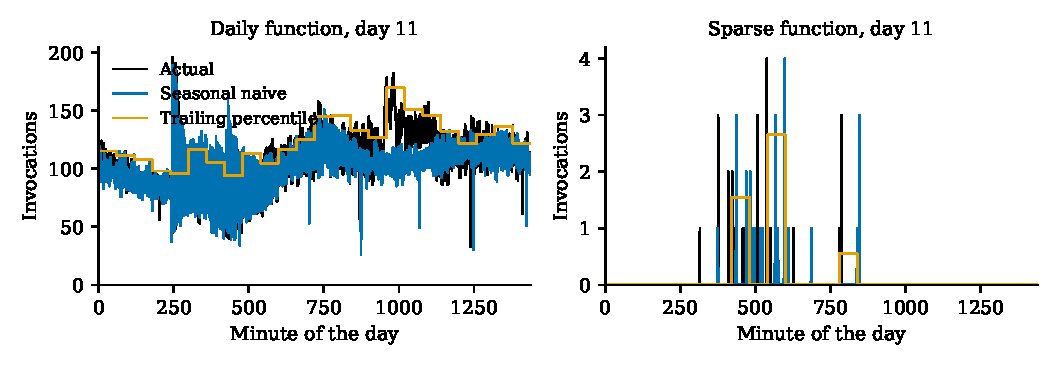
\includegraphics[width=\textwidth]{figures/forecast_examples}}
\caption{Day 11 for one daily function and one sparse function. Seasonal naive follows the daily shape. The trailing percentile stays above that shape and reacts at the sparse spikes.}
\label{fig:examples}
\end{figure*}

\begin{figure*}[t]
\centerline{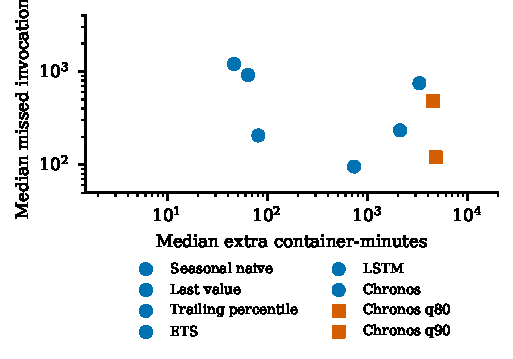
\includegraphics[width=0.86\textwidth]{figures/provisioning_tradeoff}}
\caption{Median missed invocations against median extra container-minutes on days 11--14. Both axes are logarithmic. Orange squares are Chronos forecasts at the 80th and 90th percentiles. Closer to the lower left is better.}
\label{fig:tradeoff}
\end{figure*}

\begin{table*}[t]
\caption{Held-out medians on days 13--14. The rule uses seasonal Holt--Winters for sparse functions and the trailing percentile otherwise.}
\label{tab:heldout}
\centering
\footnotesize
\begin{tabular}{|l|l|r|r|r|}
\hline
\textbf{Policy} & \textbf{Class} & \textbf{sMAPE (\%)} & \textbf{Missed} & \textbf{Extra} \\
\hline
Selection rule & Sparse & 111.6 & 0.0 & 1598.5 \\
 & Daily & 134.5 & 12.6 & 2278.5 \\
 & Bursty & 52.5 & 122.8 & 722.5 \\
 & Other & 10.8 & 56.0 & 31.5 \\
 & All & 49.9 & 16.6 & 1117.0 \\
\hline
Always seasonal naive & Sparse & 0.1 & 0.0 & 0.5 \\
 & Daily & 4.0 & 41.5 & 21.0 \\
 & Bursty & 14.2 & 361.5 & 258.0 \\
 & Other & 9.3 & 133.0 & 39.0 \\
 & All & 2.7 & 40.0 & 15.0 \\
\hline
Always trailing percentile & Sparse & 0.1 & 2.0 & 0.0 \\
 & Daily & 134.5 & 12.6 & 2278.5 \\
 & Bursty & 52.5 & 122.8 & 722.5 \\
 & Other & 10.8 & 56.0 & 31.5 \\
 & All & 16.2 & 21.0 & 120.5 \\
\hline
\end{tabular}
\end{table*}

\section{Conclusion}
\label{sec:conclusion}
On this trace, copying the previous day is the accurate forecast, including for functions whose shape repeats every day. Seasonal Holt--Winters, Chronos-Bolt, and a small LSTM all receive that same day and remain well above the copy on error. The trailing percentile misses fewer invocations because it keeps spare containers. A shortfall-only rule selects seasonal smoothing for sparse functions on a margin of 0.2 invocations and, on held-out days, spends about 1,600 extra container-minutes for no shortfall gain. A next measurement is to replace the capacity assumption with cold starts recorded on a real platform.

\bibliographystyle{IEEEtran}
\bibliography{references}

\end{document}
